\documentclass{article}
\usepackage{latexsym}
\usepackage[utf8]{inputenx}
\usepackage[spanish]{babel}
\usepackage{graphicx}
\usepackage{anysize}
\usepackage{amsmath}
\usepackage{amssymb}
\usepackage{float}
\usepackage{fancyhdr}
\setlength{\skip\footins}{5cm}
\usepackage{lscape}
\usepackage{verbatim}
\usepackage{moreverb}
\usepackage{url}
\usepackage{enumitem}
\usepackage{multicol}
\usepackage{pifont}
\let\verbatiminput=\verbatimtabinput
\usepackage[nottoc,numbib]{tocbibind}
\setcounter{tocdepth}{4}
\setcounter{secnumdepth}{4}

\marginsize{2cm}{2cm}{.5cm}{3cm} 
\pagestyle{myheadings}
\renewcommand{\headrulewidth}{0.5pt}
\begin{document}

\begin{titlepage}

\newcommand{\HRule}{\rule{\linewidth}{0.5mm}} % Defines a new command for the horizontal lines, change thickness here

\center % Center everything on the page
 
%----------------------------------------------------------------------------------------
%	HEADING SECTIONS
%----------------------------------------------------------------------------------------

\textsc{\LARGE Universidad De Buenos Aires}\\[1.5cm] % Name of your university/college
\textsc{\Large Facultad De Ingeniería}\\[0.5cm] % Major heading such as course name
\textsc{\large 75.52 Taller de Programaci\'on II}\\[0.5cm] % Minor heading such as course title

%----------------------------------------------------------------------------------------
%	TITLE SECTION
%----------------------------------------------------------------------------------------

\HRule \\[0.4cm]
{ \huge \bfseries Recursos}\\ Capa de Negocios\\[0.4cm] % Title of your document
\HRule \\[1.5cm]
 
%----------------------------------------------------------------------------------------
%	AUTHOR SECTION
%----------------------------------------------------------------------------------------

% If you don't want a supervisor, uncomment the two lines below and remove the section above
\Large \emph{Integrantes:}\\

Hugo \textsc{Chavar} - 90541\\ % Your name
Dami\'an \textsc{Manoff} - 93169\\ % Your name
Yamila \textsc{Glinsek} - 93219\\ % Your name
Andr\'es \textsc{Sanabria} - 93403\\[5cm] % Your name

\textit{capanegocio.recursos@yahoo.com.ar}
%----------------------------------------------------------------------------------------
%	DATE SECTION
%----------------------------------------------------------------------------------------

{\large \text \em \today }\\[3cm] % Date, change the \today to a set date if you want to be precise
%{10 de Septiembre de 2013}
 
%----------------------------------------------------------------------------------------

\vfill % Fill the rest of the page with whitespace

\end{titlepage}
\tableofcontents
\newpage
\section{Introducci\'on}
Recursos da referencia a lo que podemos traducir como Archivos, Links y Encuestas.\\
Los servicios que brindamos son:
\begin{enumerate}
	\item Posibilitar la subida y descarga de archivos al sistema.
	\item Crear encuestas, que pueden ser o no \emph{Evaluadas}.
	\item Permitir el acceso a responder encuestas y realizar su evaluaci\'on seg\'un el criterio establecido por el creador de la misma.
	\item Linkear p\'aginas externas y/o internas de la web.
\end{enumerate}
\markboth{Capa Negocio}{Capa Negocio- Recursos/Materiales - Grupo 2 - Tp Taller II - v 1.0}	
\section{Definiciones}
\begin{description}
	\item Cosas que ya se han definido hasta el momento por la interacci\'on con los grupos y docentes:
	\renewcommand{\labelitemi}{\ding{85}} 
	\begin{itemize}
		\item Se utilizar\'a como IDE \emph{Eclipse} y plataforma \emph{Java 7}.
		\item La comunicaci\'on entre capas se realiza por Web Services.
		\item Los archivos van a ser pasados entre capas como multi-part (o similar) a trav\'es de dichos Web Services.
		\item Tanto con la capa de arriba (Presentaci\'on) como la de abajo (Integraci\'on) implementar\'an la interfaz en XML.
		\item Los archivos ser\'an pasados de nuestra capa a la  \emph{capa de Integraci\'on}  para que \'esta trate con el FileSystem o con la \emph{capa de Acceso a datos} como ha de ser almacenado. Queda por definirse si es necesario una conversaci\'on previa entre capas antes de la transferencia del archivo.
%\item 

	\end{itemize}


\end{description}

\markboth{Capa Negocio}{Capa Negocio- Recursos/Materiales - Grupo 2 - Tp Taller II - v 1.0}	
\section{Diagrama de Clases}
	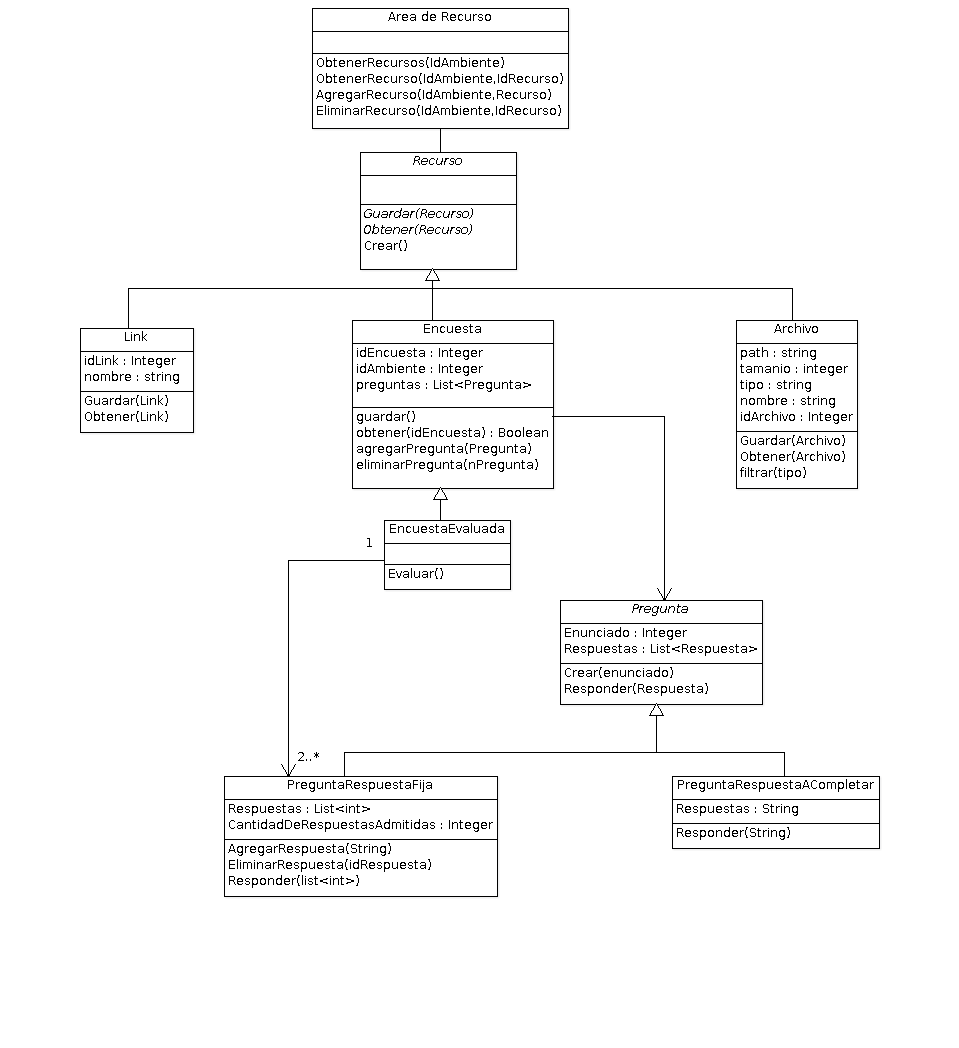
\includegraphics[scale=0.5]{Diagramadeclase2copia.png}
\markboth{Capa Negocio}{Capa Negocio- Recursos/Materiales - Grupo 2 - Tp Taller II - v 1.0}	
\pagebreak
	

\section{Interfaces}
	\begin{description}
		\item[Provistas a la capa de Presentaci\'on  \emph{( incompleto)}] \
		\renewcommand{\labelitemi}{\ding{105}} 
		\begin{itemize}
			\item \emph{CARGAR LISTA RECURSOS}
			\begin{description}
				\item[INPUT] ID-AMBIENTE
				\item[OUTPUT] LISTA-DE [ID-RECURSO, DESCRIPCION, TIPO]
			\end{description}
			\item \emph{OBTENER RECURSO}
			\begin{description}
				\item[INPUT] ID-AMBIENTE, ID-RECURSO
				\item[OUTPUT] LINK-AL-RECURSO \'o ARCHIVO \'o ACCESO-A-ENCUESTA
			\end{description}
			\item \emph{AGREGAR RECURSO}
			\begin{description}
				\item[INPUT] ID-AMBIENTE, DESCRIPCI\'ON, DATOS (\emph{Difiere seg\'un tipo de recurso})
				\item[OUTPUT] MENSAJE DE CONFIRMACI\'ON
			\end{description}
			\item \emph{BORRAR RECURSO}
			\begin{description}
				\item[INPUT] ID-AMBIENTE, ID-RECURSO
				\item[OUTPUT] MENSAJE DE CONFIRMACI\'ON
			\end{description}
		\end{itemize}
		\renewcommand{\labelitemi}{\ding{118}} 
		\item[Requeridas a la capa de Integraci\'on \emph{( incompleto)}] \
		\\Nota:
		\emph{ En un principio, no necesitaremos que la capa de integraci\'on haga joins de tablas de Base de Datos, ya que todo va a ser requerido por ID.}
		\begin{itemize}
			\item \emph{OBTENER LISTA RECURSOS}
			\begin{description}
				\item[INPUT] ID-AMBIENTE
				\item[OUTPUT] LISTA-DE [ID-RECURSO, DESCRIPCION, TIPO]
			\end{description}
			\item \emph{OBTENER RECURSO}
			\begin{description}
				\item[INPUT] ID-AMBIENTE, ID-RECURSO
				\item[OUTPUT] LINK-AL-RECURSO
			\end{description}
			\item \emph{OBTENER ARCHIVO}
			\begin{description}
				\item[INPUT] LINK-AL-ARCHIVO
				\item[OUTPUT] ARCHIVO
			\end{description}
			\item \emph{AGREGAR RECURSO}
			\begin{description}
				\item[INPUT] ID-AMBIENTE, DESCRIPCI\'ON, TIPO, DATOS (\emph{Difiere seg\'un tipo de recurso})
				\item[OUTPUT] MENSAJE DE CONFIRMACI\'ON \'o LINK-AL-RECURSO
			\end{description}
			\item \emph{BORRAR RECURSO}
			\begin{description}
				\item[INPUT] ID-AMBIENTE, ID-RECURSO
				\item[OUTPUT] MENSAJE DE CONFIRMACI\'ON
			\end{description}
		\end{itemize}
	\end{description}
	\markboth{Capa Negocio}{Capa Negocio- Recursos/Materiales - Grupo 2 - Tp Taller II - v 1.0}
\end{document}
